Before presenting our methods in Section~\ref{sect:method}, we first compare composition architectures that invoke either SLMs (typically mid-performing) or frontier LLMs, in order to highlight the performance gap within prior discussion-based architectures. Specifically, we evaluate three discussion-based composition architectures: LLM-Debate~\citep{du2023improvingfactualityreasoninglanguage}, Mixture-of-Agents~\citep{wang2024mixtureofagentsenhanceslargelanguage}, and Multi-Agent Verification~\citep{lifshitz2025multiagentverificationscalingtesttime}. We use the same experimental settings for SLMs and frontier LLMs; we vary only the choice of models between a small-sized group and a frontier (often larger) group.

As shown in Figure~\ref{fig:small-large-accuracy}, discussion-based architectures generally outperform the single best-performing models in the frontier LLM group, achieving up to a 2\% increase in accuracy. However, when applied to SLMs, these discussion-based architectures fail to outperform the best single model in the composition, and even incur accuracy drops of up to 5.5\%. This performance gap is observed across all three methods and both benchmarks. This raises a central question: are existing discussion-based architectures truly suitable for SLMs?

% In this section, we conduct an thorough evaluation and analysis existing LLM combination methods. While existing LLM combination methods (such as LLM-debate, multi-agent verification) show good performance gain, they usually directly utilize frostier models such as GPT 3.5 and GPT 4. Given larger models usually have a better pretraining volume and cognitive ability, they usually benefit from discussing with each other. It is worth questioning that if these methods will still hold true under small models settings, where models have limited knowledge and generally weak cognitive ability.    

% As shown in Figure~\ref{fig:small-large-accuracy}, existing combination methods consistently yield superior performance for large-sized, frontier models, often outperforming any individual model. However, when applied to smaller-scale models, these methods fail to deliver gains over the strongest individual model, despite incurring substantial computational and token usage costs due to multiple model queries. Existing combination methods that is based on text communication between models are ineffective when using small-scaled, mediocre-performing language models.

% To analyze why this ineffectiveness happens, we further investigate into the failure cause of the methods.

% This observation underscores a key limitation: compositional methods that rely on iterative reasoning or multi-step interactions exhibit a strong dependency on the underlying model's capabilities. In the case of smaller-scale models, the additional rounds of reasoning do not lead to higher accuracy. Instead, accuracy often plateaus or even degrades, suggesting that interaction-based composition may not be suitable for resource-constrained or lower-capacity models.


\begin{figure}[htbp]
  \centering
  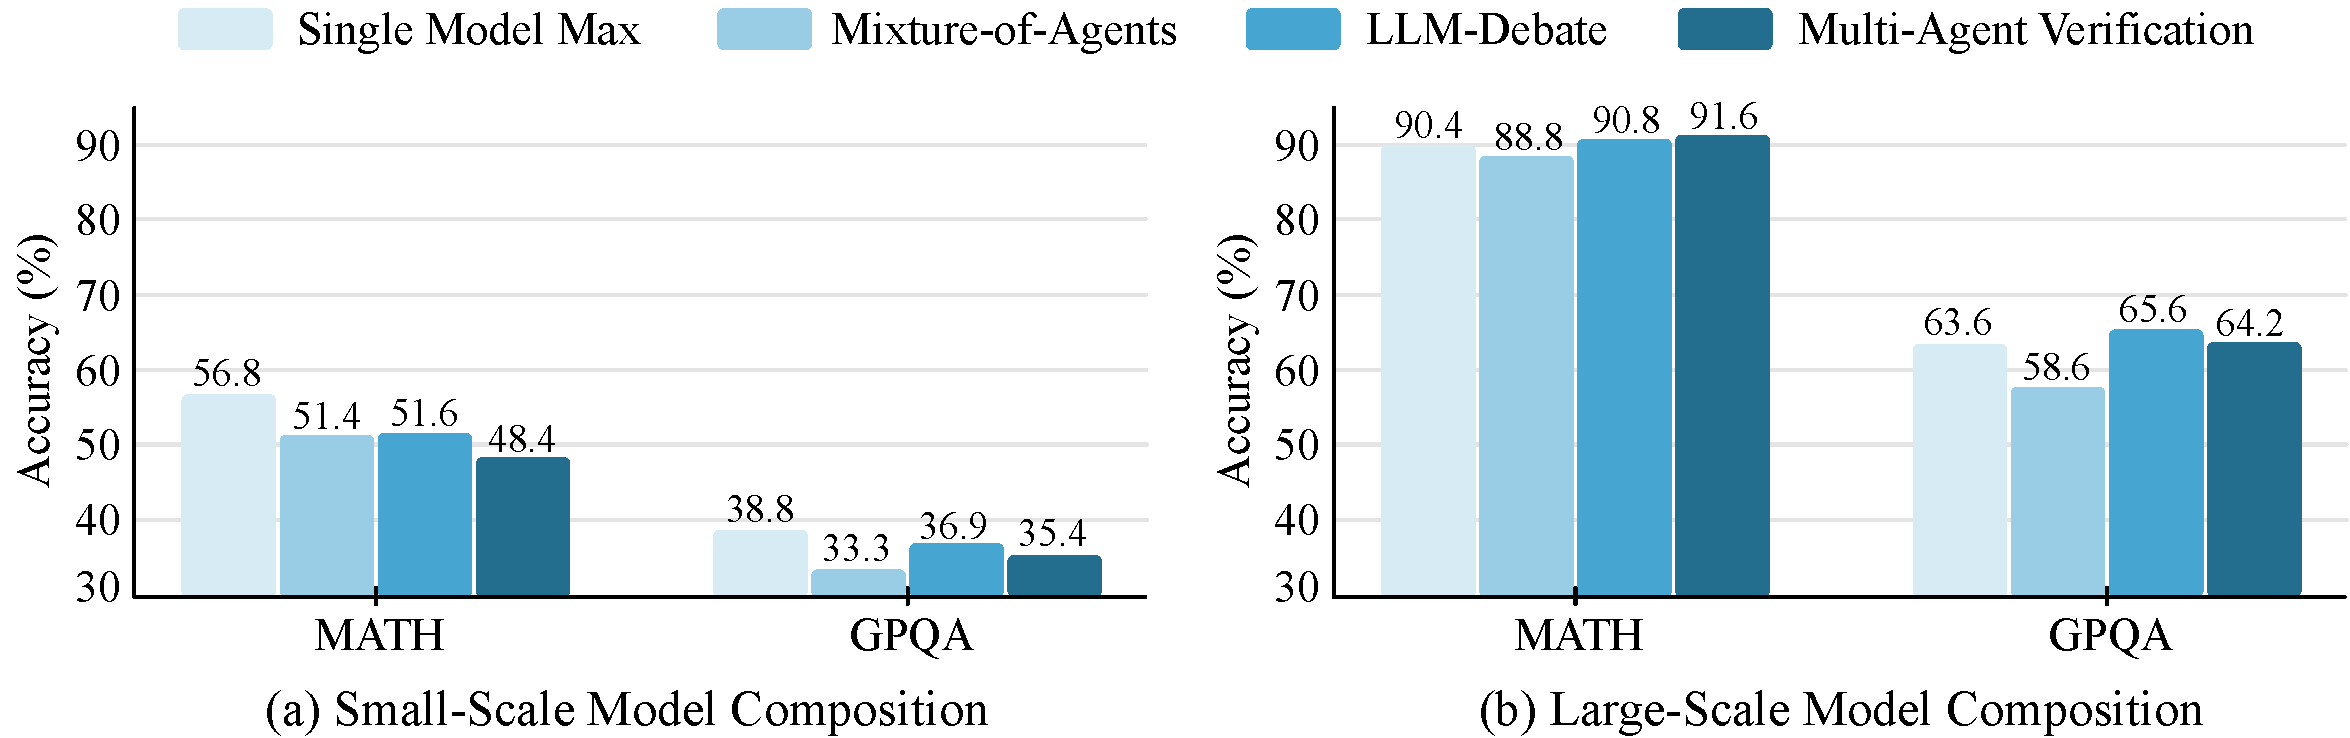
\includegraphics[width=0.9\linewidth]{Figures/Small-large-acc-light-blue_v2.pdf}
  \vspace{-8pt}
  \caption{\small \textbf{Comparison of discussion-based orchestration when invoking SLMs and LLMs.} We compare three compositional architectures (Mixture-of-Agents, LLM-Debate, and Verification) using (a) SLMs (Llama 3.1 8B, Mistral 8$\times$7B, Gemma 2 27B) and (b) frontier LLMs (DeepSeek V3, Gemini 2.0 Flash, GPT-4o) on the \textsc{MATH} and \textsc{GPQA} datasets. The baseline (\textit{Single-Model Max}) reflects the best performance of individual models. A composition is considered successful if it surpasses Single-Model Max.}\label{fig:small-large-accuracy}
  \vspace{-10pt}
\end{figure}


% To understand why compositional methods underperform with smaller language models, we conducted a detailed diagnostic analysis of representative failure cases using the LLM-Debate method~\cite{du2023improving}. Specifically, we examined dialogue transcripts from model interactions on the MATH dataset involving computationally efficient models (Mistral-8$\times$7B, LLaMA-3.1-8B, Gemma-2-27B). Our analysis revealed two overarching categories of failure:

To better understand this gap, we analyze the behavior of SLMs. Our findings highlight a key limitation: rather than correcting mistakes, discussion-based methods often amplify them. Our two observations support this claim: (1) when prompting an LLM to explain failures in the debate setting, we find that the discussions tend to reinforce incorrect reasoning rather than resolve it. (2) From a statistical perspective, we observe that SLMs tend to adopt the answer most recently presented in the context, rather than reviewing and reflecting on the entire discussion. More details of this analysis are presented in the Appendix.

Together, these observations suggest that existing discussion-based frameworks are ill-suited for SLMs. Their limited reasoning capacity necessitates a new composition architecture, which we will present in Section~\ref{sect:method}.


% \begin{figure}[t]
%   \centering
%   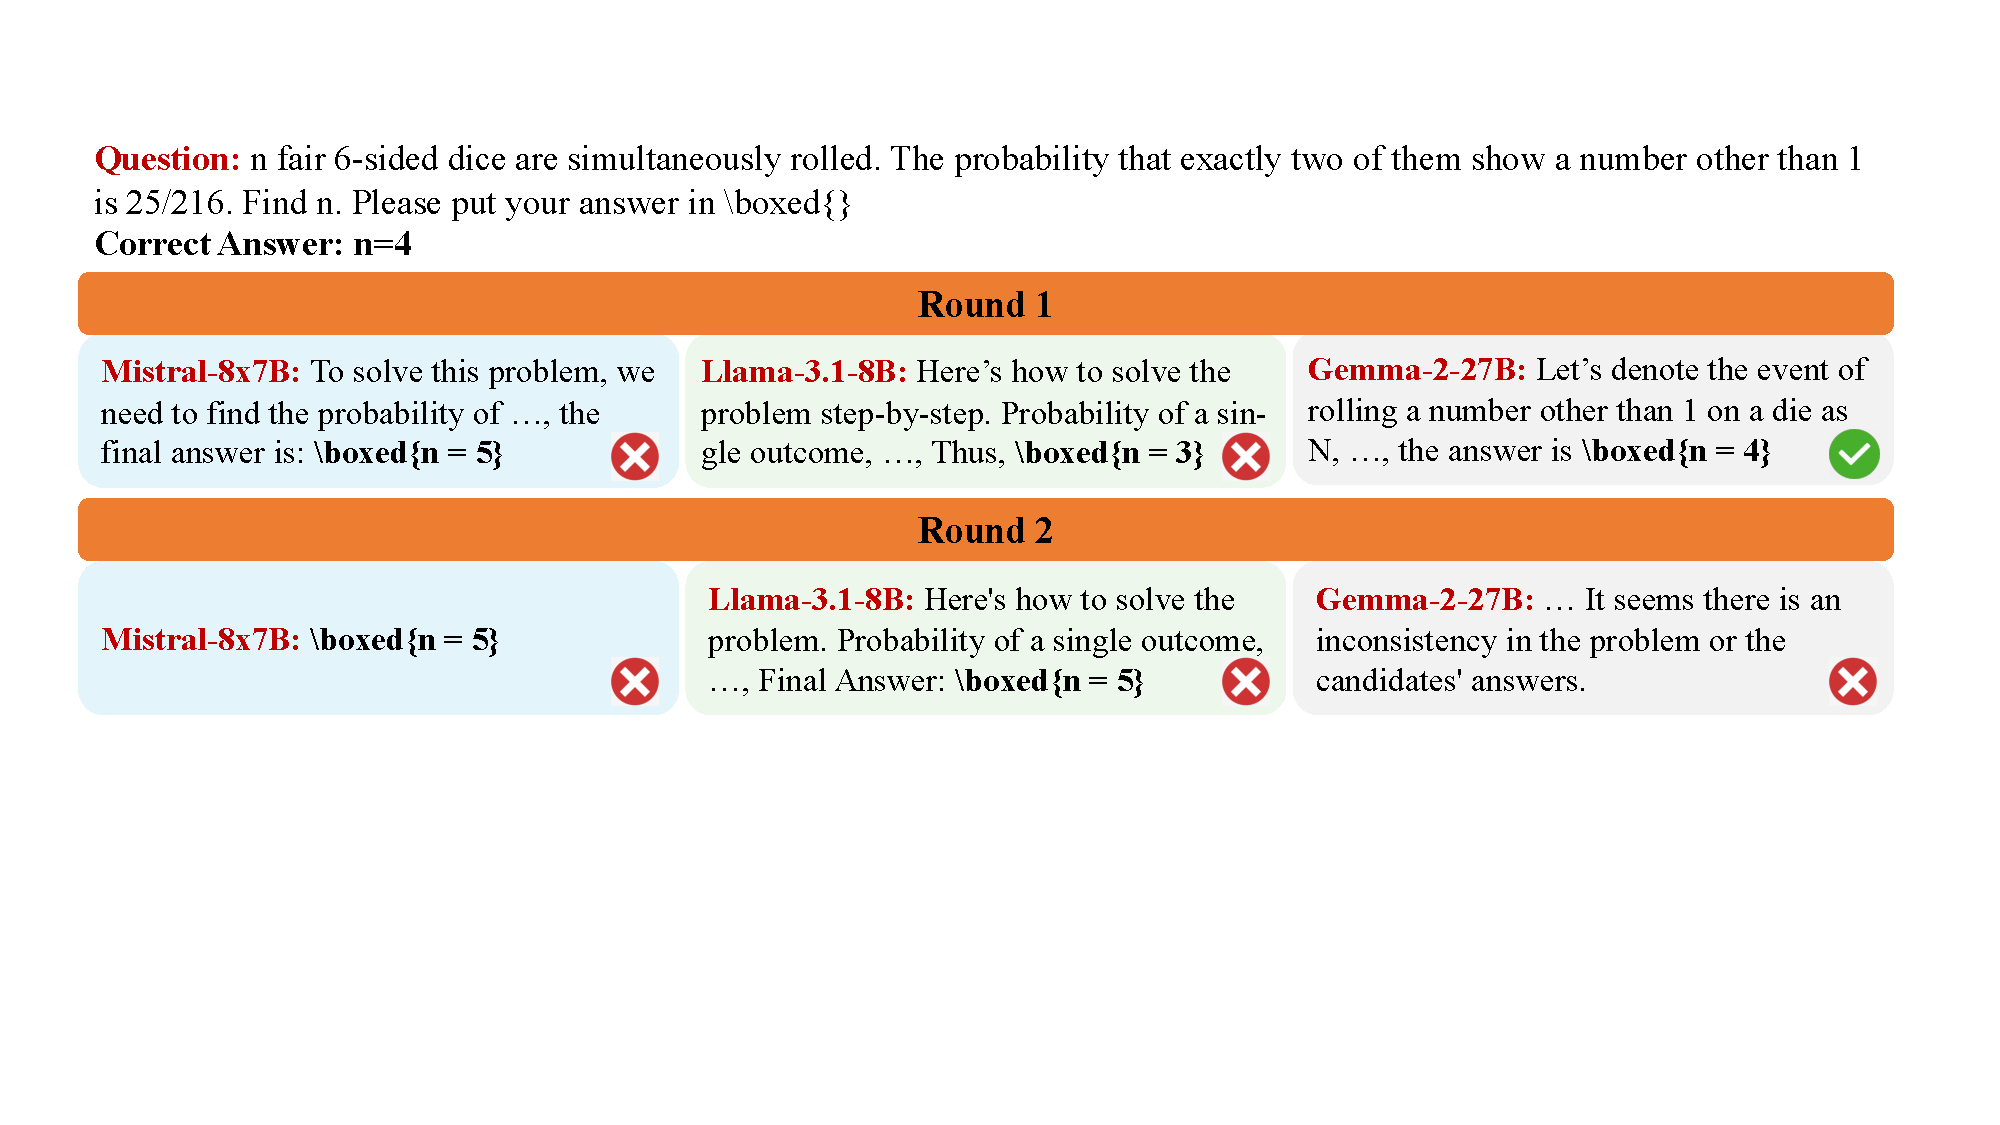
\includegraphics[width=\linewidth]{Figures/failure_case_interaction.pdf}
%   \vspace{-10pt}
%   \caption{\small \textbf{Illustration of Superficial Interactions.} A failure case illustrating ineffective interaction in a small-model debate setting. Model 1 simply repeated its previous answer without any additional reasoning.}
%   \vspace{-5pt}
%   \label{fig:fail-case}
% \end{figure}

% \paragraph{Superficial Interactions.} 
% A significant failure mode involves superficial engagement, which can manifest in various unproductive behaviors during debates. For instance, models sometimes simply repeat previous answers without genuine reconsideration or reflection, ignoring the debate's iterative nature and the expectation to refine their responses. Other models may merely critique perceived inconsistencies or errors in peer responses without contributing substantive new ideas or solutions. Occasionally, models revert to earlier solutions for verification without progressing further, failing to advance the discussion. Additionally, certain models may incorporate flawed elements from peer answers directly into their own revised solutions, unintentionally propagating errors rather than correcting them. These types of superficial and non-reflective interactions collectively undermine the intended dynamic and progressive nature of debate methodologies.

% Figure~\ref{fig:fail-case} illustrates a representative example of superficial engagement. In Round 1, three models respond to a probability problem involving dice rolls: Model 1 and Model 2 produce incorrect answers, while Model 3 identifies the correct solution. However, during Round 2, rather than engaging deeply with each other's reasoning as intended, Model 1 merely repeats its initial incorrect response without any further reasoning. Model 2, influenced negatively by Model 1, shifts from one incorrect answer to another without genuinely incorporating the correct insight from Model 3. Model 3, despite having provided the correct solution initially, deviates from the task in Round 2 by critiquing the inconsistencies of the other models rather than reaffirming or further elaborating its original correct response. This leads Model 3 to abandon its initial correct answer, demonstrating the superficial level of engagement that inhibits effective debate and knowledge integration among models.


% \paragraph{Intrinsic Capability Limitations.} 
% % Another important limitation is related to the intrinsic abilities of smaller models. This limitation does not seem to be related to the interactions between models, but rather because of their inherent limitations. For example, smaller models often have difficulty placing their answers exactly where we expect them, especially as the context grows longer. Additionally, all models sometimes struggle to identify the common error in their answers, even after debate.
% Another critical challenge arises from the inherent limitations of smaller language models, independent of their interactions with other agents. These limitations often manifest as difficulties in adhering to formatting expectations or in maintaining reasoning consistency, especially as prompt contexts grow longer. For instance, smaller models frequently misplace final answers or fail to follow explicitly specified output structures. Additionally, even after multiple rounds of debate, models often struggle to recognize and correct common reasoning errors, highlighting fundamental constraints in their self-correction capabilities.

% \begin{figure}[htbp]
%   \centering
%   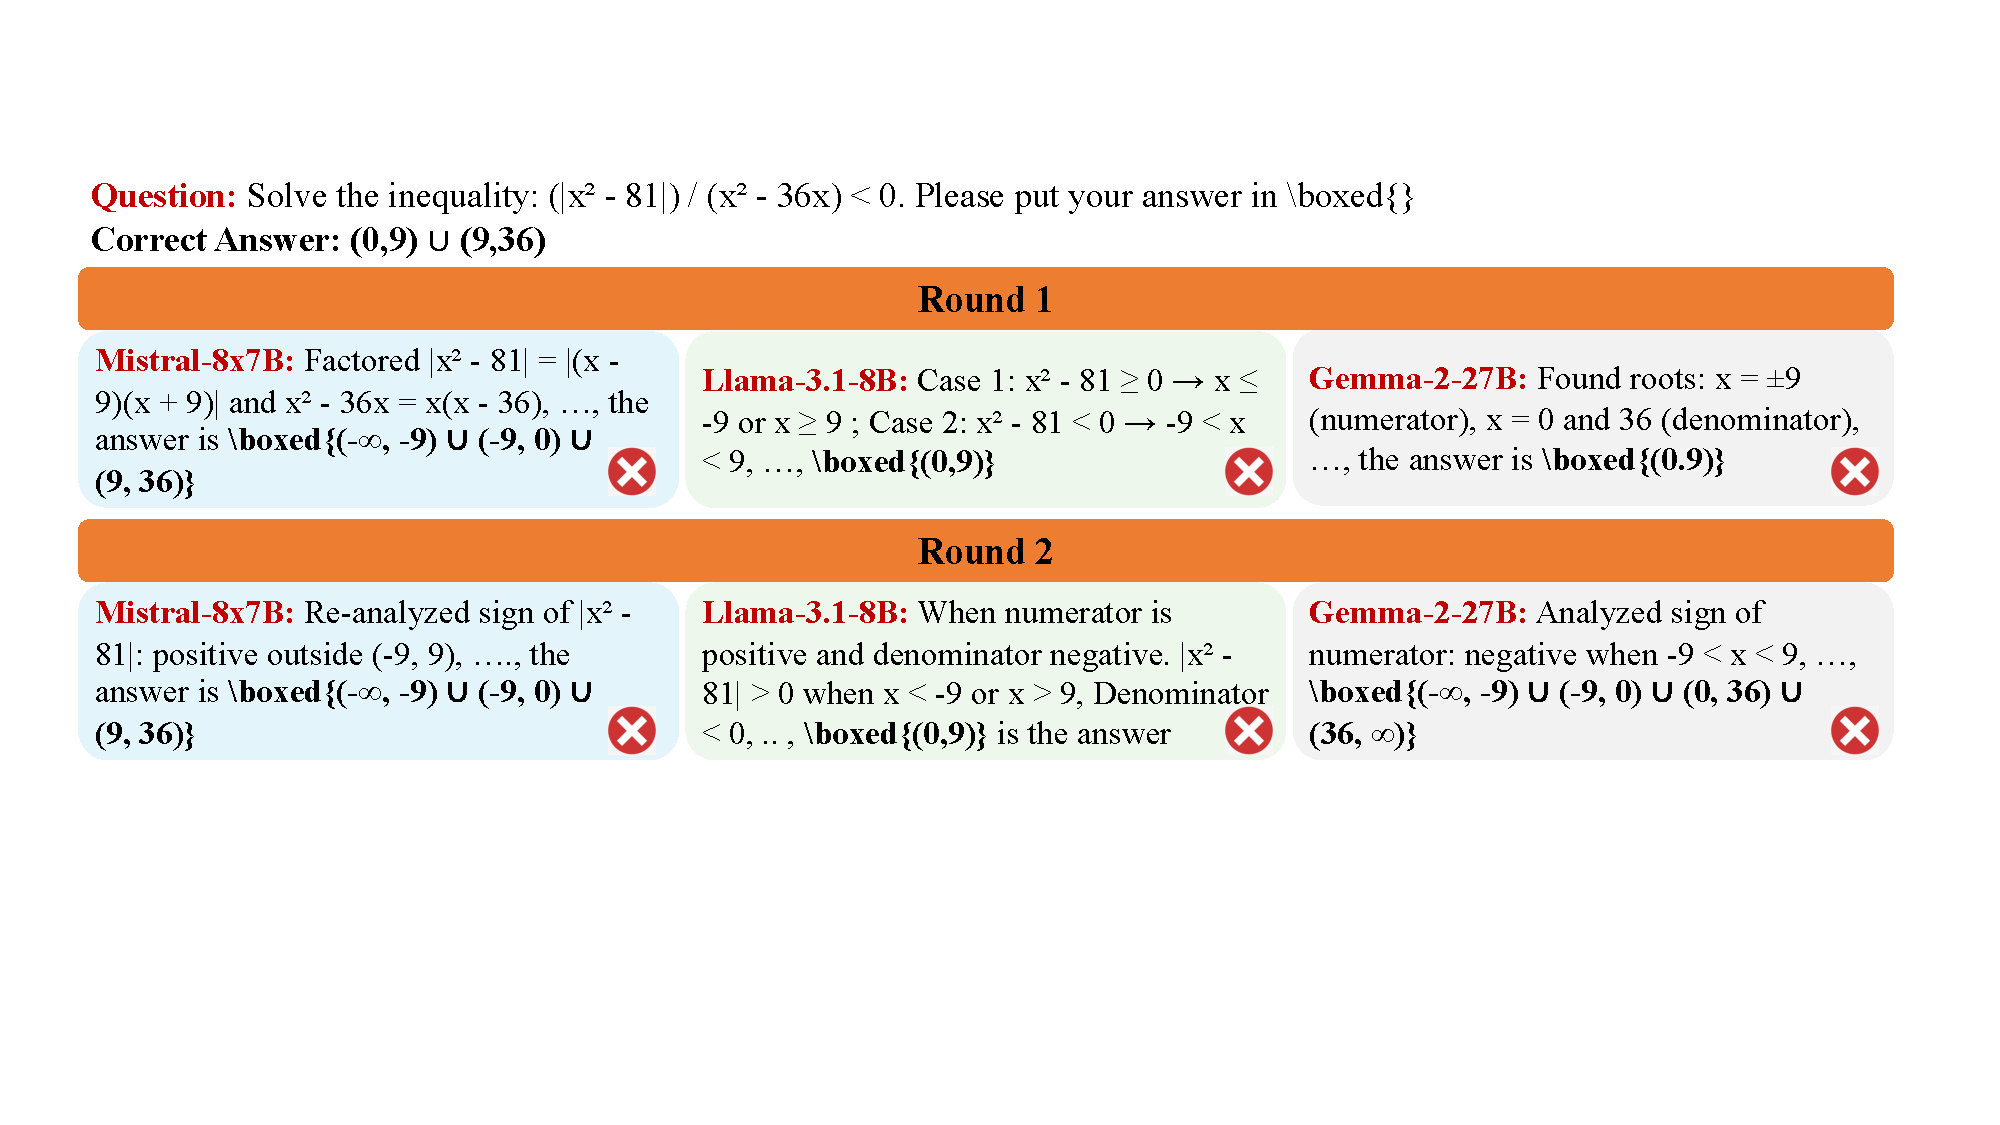
\includegraphics[width=\linewidth]{Figures/failure_case_model_capability.pdf}
%   \vspace{-10pt}
%   \caption{\small \textbf{Illustration of Intrinsic Capability Limitations.} A failure case illustrating an intrinsic capability limitation of the model. The model failed to correctly identify the conditions of the problem and did not place the solution in the prompt-specified location. For clarity and conciseness, we summarize the reasoning process.}
%   \label{fig:fail-case-2}
%   \vspace{-15pt}
% \end{figure}

% % Figure~\ref{fig:fail-case-2} illustrates an intrinsic capability limitation observed in small models. Specifically, in this example, the models failed to accurately determine the sign intervals of the numerator and denominator during the problem-solving process, leading to incorrect identification of the function's sign and thus incorrect solution intervals. All models fail to correct this mistake after the debate. Additionally, model 2 did not correctly place the final answer in the explicitly specified location, complicating the extraction of the solution. Although misplacement of answers might seem minor, such errors frequently occur and significantly impact the overall effectiveness of small-model compositions.

% Figure~\ref{fig:fail-case-2} presents an example of such intrinsic limitations. In this case, all models fail to correctly identify the sign intervals of the numerator and denominator, resulting in an incorrect determination of the function’s sign and solution intervals. Despite the opportunity for collaborative correction during debate, the error persists across all responses. Moreover, Model 2 fails to place the final answer in the designated location, making the solution harder to extract—an issue that, while seemingly minor, frequently undermines the practical utility of small-model outputs in compositional workflows.

% Interestingly, we observe that smaller models perform consistently well when responding directly to prompts. Although their answers are not always accurate, the errors typically stem from knowledge or reasoning limitations rather than misunderstandings of prompt structure or formatting. This contrast highlights that the core challenges lie not in instruction-following ability, but in the models’ limited capacity to handle complex reasoning tasks and participate effectively in multi-agent interactions.